\documentclass[11pt, ngerman]{article}
\usepackage{cite}
\usepackage{url}
\usepackage{amsmath}
\usepackage{amsfonts}
\usepackage{cleveref}
\usepackage{xstring}
\usepackage{trfsigns}
\usepackage{verbatim}
\usepackage{listings}
\usepackage{graphicx}
\usepackage{xcolor}
\usepackage{caption}
\usepackage{float}


\crefname{equation}{Gleichung}{Gleichungen}

\lstset{breaklines=true,language=C, keywordstyle=\color{blue}, morekeywords={kernel, global, local, constant, const}}

\begin{document}

\newcommand*{\Ef}[3]{%
	\IfEqCase{#3}{%
		{+}{E_{#1}^{#2}\vert_{t+\Delta t}}%
		{-}{E_{#1}^{#2}\vert_{t-\Delta t}}%
		{0}{E_{#1}^{#2}\vert_{t}}%
		{T}{E_{#1}^{#2}\vert_{T}}%
	}[\PackageError{tree}{Undefined option to Ef: #1}{}]%
}

\newcommand*{\Hf}[3]{%
	\IfEqCase{#3}{%
		{+}{\widetilde{H_{#1}}^{#2}\vert_{t+\frac{\Delta t}{2}}}%
		{-}{\widetilde{H_{#1}}^{#2}\vert_{t-\frac{\Delta t}{2}}}%
		{0}{\widetilde{H_{#1}}^{#2}\vert_{t}}%
		{T}{\widetilde{H_{#1}}^{#2}\vert_{T}}%
	}[\PackageError{tree}{Undefined option to Hf: #1}{}]%
}

\newcommand*{\Ch}[3]{%
	\IfEqCase{#3}{%
		{+}{C_{#1}^H\vert_{t+\frac{\Delta t}{2}}^{#2}}%
		{-}{C_{#1}^H\vert_{t-\frac{\Delta t}{2}}^{#2}}%
		{0}{C_{#1}^H\vert_{t}^{#2}}%
		{T}{C_{#1}^H\vert_{T}^{#2}}%
		{T+}{C_{#1}^H\vert_{T+\frac{\Delta t}{2}}^{#2}}%
	}[\PackageError{tree}{Undefined option to Cf: #1}{}]%
}

\newcommand*{\Ce}[3]{%
	\IfEqCase{#3}{%
		{+}{C_{#1}^E\vert_{t+\frac{\Delta t}{2}}^{#2}}%
		{-}{C_{#1}^E\vert_{t-\frac{\Delta t}{2}}^{#2}}%
		{0}{C_{#1}^E\vert_{t}^{#2}}%
		{T}{C_{#1}^E\vert_{T}^{#2}}%
		{T+}{C_{#1}^E\vert_{T+\frac{\Delta t}{2}}^{#2}}%
	}[\PackageError{tree}{Undefined option to Cf: #1}{}]%
}

\newcommand*{\dt}[3]{%
	\begin{bmatrix}
		{#1} & 0 & 0\\
		0 & {#2} & 0\\
		0 & 0 & {#3}
	\end{bmatrix}
}

\newcommand*{\sgma}{\sigma^`}
\newcommand*{\sollsein}{\stackrel{!}{=}}

\newcommand*{\mone}{\frac{\sgma_y+\sgma_z}{2\epsilon_0} + \frac{\sgma_y\sgma_z\Delta t}{4\epsilon_0} + \frac{1}{\Delta t}}
\newcommand*{\fone}{-\frac{\sgma_y+\sgma_z}{2\epsilon_0} + \frac{\sgma_y\sgma_z\Delta t}{4\epsilon_0} + \frac{1}{\Delta t}}

\newcommand{\source}[1]{\caption*{Source: {#1}} }


\title{Hardwarebeschleunigte Simulation von Drahtantennen}
\author{Lukas Brumm (S553370)}
\date{\today}
\maketitle
\newpage

\section{Einleitung}
% Jede drahtlose Kommunikation benoetigt eine Antenne auf der
% Sende- und der Empfangsseite, diese muss haeufig besondere
% Eigenschaften, wie zum Beispiel eine besondere Abstrahlcharakteristik
% aufweisen, oder muss besonders klein sein. Der Entwurf einer solchen
% Antenne ist analytisch nicht moeglich sonder passiert computergestuetzt
% durch ein Simulationsprogramm. Ein solches Simulationsprogramm loest
% die Maxwellgleichungen numerisch unter Beruecksichtigung der eingegebenen
% Randbedingungen. Eine Moeglichkeit die Maxwellgleichungen zu loesen
% ist die Methode der finiten Differenzen im Zeitbereich (FDTD), die in
% der folgenden Arbeit erlaeutert wird.
% Weiterhin wird die FDTD hardwarebeschleunigt implementiert, da eine
% performante Simulation von Antennen die Verwendung von evolutionaeren
% Algorithmen zum automatisierten Antennendesign ermoeglichen sollte.
Die vorliegende Arbeit "Hardwarebeschleunigte Simulation von Drahtantennen"
wurde im Rahmen des Studienganges `Informations- und 
Kommunikationstechnik' an der Hochschule fuer Technik und Wirtschaft Berlin
(HTW) verfasst. Ziel der Arbeit ist es die Methode der finiten Differenzen
im Zeitbereich (FDTD-Methode) nachzuvollziehen und fuer eine
hardwarebeschleunigte Simulation von Drahtantennen zu verwenden.
Da numerische Loesungsverfahren fuer Differentialgleichunen nicht
Teil meines Studiums waren hiehlt ich mich bei der Herleitung der FDTD-Methode
an die Vorlesung `Electromagnetic Analysis Using Finite-Difference Time-Domain'
samt veroeffentlichtem Skript Raymond Rumpfs der Universitaet
Texas in El Paso, wobei ich mich entschloss die Maxwellgleichungen fuer
ein normalisiertes H-Feld zu loesen und nur auf dem E- und H-Feld zu arbeiten.
Dadurch laesst sich die numerische Loesung der Maxwellgleichungen
durch nur zwei Formeln gaenzlich beschreiben.

\section{Motivation}
Jede drahtlose Kommunikation benoetigt eine Antenne auf der
Sende und Empfangsseite. Durch die Fortschreitende Miniaturisierung
der Elektronik und eine daraus folgende Vernetzung 
wie man sie zum Beispiel im Internet of Things (IoT)
beobachten kann werden immer spezifischere Charakteristiken
an die Sende- und Empfangsantenne gestellt. In solchen Einsatzgebiete
sind konventionelle Antennendesigns haeufig nicht anwendbar,
sondern erfordern spezielle Antennen. Der Entwurf solcher Antennen
passiert interaktiv mit einem Simulationsprogramm, wobei auch
gezeigt wurde, dass evolutionaere Algorithmen (EA) zum automatisierten
Antennendesign verwendet werden koennen.\cite{nasa_ea_antenna}
Ein solcher EA muss mitunter hunderttausende Simulationen durchfuehren\cite[p.6]{nasa_ea_antenna},
weshalb jede Simulation so performant wie moeglich sein sollte.

\section{Stand der Technik}
Das numerische Loesen von Differentialgleichungnen wird seit 1928 untersucht
\cite{fdtd_u} und hat sich seitdem kontinuierlich weiterentwickelt.\cite{fdtd_history}
Neben der FDTD existieren noch andere Verfahren um Differentialgleichungen
zu loesen wie zum Beispiel die Finite-Elemente-Methode, die Finite-Volumen-Methode,
oder die Randelement-Methode, die haeufig fuer Differentialgleichungen
besonderer Form entwickelt wurde.\cite{mathepedia_numerische_verfahren} 
Die FDTD-Methode hingegen kann auf beliebige Differentialgleichungen angewandt
werden und wird im Verlaufe der Arbeit eingehend behandelt.
Auch wenn die FDTD-Methode seit 1928 erforscht wird werden fuer die Einsatzgebiete
der FDTD neue Erkenntisse gewonnen, so ist die Simulation einer Antenneneinspeisung
noch nicht vollstaendig geklaert und wird weiterhin untersucht.\cite{advanced_gap_feed}

\section{Loesen der Maxwellgleichungen durch die FDTD-Methode}
Die FDTD-Methode, auch Yee-Methode genannt, loest Differentialgleichungen
indem die als infinitesimal klein angenommenen Differentialquotienten
durch finite Differenzenquotienten approximiert werden.~\cite{fdtd_u}
Die Maxwellgleichungen werden daher nur in der Differentialform betrachtet.
Die FDTD-Methode ist zu komplex und problemabhaengig,
als dass eine Einschaetzung der Simulationsergebnise gelingen koennte ohne die FDTD-Methode
mathematisch fuer ein Problem nachvollzogen zu haben.
Es werden daher nun kurz die Maxwellgleichungen eingefuehrt, allgemeine
Stabilitaetsbedingungen der FDTD-Methode behandelt und die FDTD-Methode
genutzt um eine numerische Loesung der Maxwellgleichungen sowie des
`Perfectly Matched Layer' (PML) herzuleiten.

\subsection{Maxwellgleichungen}
Unter den Maxwellgleichungen versteht man die folgenden Gleichungen, die
zusammen alle elektromagnetischen Phaenomene beschreiben.
Das Gausz-Gesetz fuer Elektrizitaet\cite{gausz_law_electric},

\begin{equation}
	\nabla * \vec{D} = \rho_v
	\label{eq:gausz_law_e}
\end{equation}
wobei \(\vec{D}\) die elektrische Flussdichte und \(\rho_v\) die Ladungsdichte ist.
Elektrische Felder divergieren bei positiven Ladungen und konvergieren bei negativen
Ladungen. Das Gausz-Gesetz fuer Magnetismus\cite{gausz_law_magnetic},

\begin{align}
	\nabla * \vec{B} = 0
	\label{eq:gausz_law_h}
\end{align}
wobei \(\vec{B}\) die magnetische Flussdichte ist.
Es gibt keine magnetischen Monopole, Magnetfelder formen immer Schleifen.
Das Amperesches Gesetz\cite{amperes_law},

\begin{align}
	\nabla\times\vec{H} = \vec{J} + \frac{\partial\vec{D}}{\partial t}
\end{align}
wobei \(\vec{H}\) das magnetische Feld und \(\vec{J}\) die Stromdichte ist.
Zirkulierende magnetishe Felder induzieren Stroeme sowie zeitabhaengige
elektrische Felder. Das Induktionsgesetz\cite{induction_law},

\begin{align}
	\nabla\times\vec{E} = -\frac{\partial\vec{B}}{\partial t}
\end{align}
wobei \(\vec{E}\) das elektrische Feld ist.
Zirkulierende elektrische Felder induzieren zeitabhaengige magnetische Felder.
Weiterhin ist das D-Feld ueber die Permittivitaet mit dem E-Feld verbunden,\cite{constitutive}

\begin{align}
	\vec{D}(t) = [\epsilon(t)] * \vec{E}(t)
	\label{eq:constitutive1}
\end{align}
sowie das B-Feld ueber die Permeabilitaet mit dem H-Feld verbunden ist.\cite{constitutive}

\begin{align}
	\vec{B}(t) = [\mu(t)] * \vec{E}(t)
	\label{eq:constitutive2}
\end{align}
In beiden Faellen handelt es sich um eine Faltung mit einem Tensor.
Im Verlauf der Arbeit wird angenommen, dass die Permittivitaet und die Permeabilitaet zeitlich
konstant sind. Damit wird die Faltung zu einer Multiplikation. Verwendet man die
\cref{eq:constitutive1,eq:constitutive2} um das D- und B-Feld zu eliminieren und
gibt man die Permittivitaet und Permeabilitaet relativ zur Vacuumpermittivitaet und
-permeabilitaet an so ergeben sich folgende vier Formeln.

\begin{align}
	&\nabla * ([\mu]\vec{H}(t)) = 0 \\
	&\nabla * ([\epsilon]\vec{E}(t)) = \rho_v \\
	&\nabla\times\vec{H} = \epsilon_0[\epsilon_r]\frac{\partial\vec{E}}{\partial t} \label{eq:nabla_h} \\
	&\nabla\times\vec{E} = -\mu_0[\mu_r]\frac{\partial\vec{H}}{\partial t} \label{eq:nabla_e}
\end{align}
Aus den beiden verschraenkten \cref{eq:nabla_h,eq:nabla_e} werden spaeter die sog.
Updategleichungen hergeleitet, also die Gleichungen die das E- bezw. H-Feld des naechsten
Zeitschrittes liefern. Die Stromdichte \(\vec{J}\) kann genutzt werden um
Verlust innerhalb von Materialien darzustellen. Im Verlauf der Arbeit wird angenommen,
dass die Antennengeometrie nicht verlustbehaftet ist.

\begin{align}
	\vec{J} = 0\nonumber\\
\end{align}
Das E- und H-Feld sind durch die Materialimpedanz \(\eta\) mit einander verknuepft, wobei jede
Impedanz relativ zur Freiraumimpedanz \(\eta_0\) angegeben werden kann:

\begin{align}
	\eta &= \frac{|\vec{E}|}{|\vec{H}|} \nonumber\\
	\eta &= \eta_0 * \sqrt{\frac{\mu_r}{\epsilon_r}}, \eta_0 = \pi*119,9169832\Omega
\end{align}
Im freien Raum ist das E- Feld also um den Faktor \(\eta_0\) groeszer als das H-Feld.
Diese Skalierung fuehrt bei numerischen Loesungsverfahren zu Rundungsfehlern,
weshalb das H-Feld normalisiert wird und somit die gleiche Groeszenordnung wie das
E-Feld besitzt.\cite{normalize_h_field}

\begin{align}
	\widetilde{\vec{H}} &= \eta_0\vec{H}\nonumber\\
	\vec{H} &= \frac{1}{\eta_0}\widetilde{\vec{H}}
\end{align}
Sommit ergibt sich aus \cref{eq:nabla_e}:

\begin{align}
	\nabla\times\vec{E} &= [-\mu]\frac{\partial\widetilde{\vec{H}}}{\partial t} * \frac{1}{\eta_0}\quad\vert \eta_0 = \mu_0 * c\\
	&=-\mu_0[\mu_r]\frac{1}{\mu_0c}\frac{\partial\widetilde{\vec{H}}}{\partial t}\\
	&=-\frac{[\mu_r]}{c}\frac{\partial\widetilde{\vec{H}}}{\partial t}
\end{align}
Und aus \cref{eq:nabla_h} ergibt sich:

\begin{align}
	\nabla\times\widetilde{\vec{H}} &= \eta_0\epsilon_0[\epsilon_r]\frac{\partial\vec{E}}{\partial t}\\
	&= c\mu_0\epsilon_0[\epsilon_r]\frac{\partial\vec{E}}{\partial t}\quad\vert \mu_0 = \frac{1}{c^2\epsilon_0}\\
	&= \frac{1}{c^2\epsilon_0}c\epsilon_0[\epsilon_r]\frac{\partial\vec{E}}{\partial t}\\
	&= \frac{[\epsilon_r]}{c}\frac{\partial\vec{E}}{\partial t}
\end{align}


\subsection{Mathematische Stabilitaetsbedingungen fuer finite Differenzen}
Immer wenn die FDTD-Methode auf Differentialgleichungen angewendet
wird muss jede finite-Differenz am selben Punkt im Raum und in der
Zeit existieren um die Differentialgleichung korrekt zu approximieren.\cite{fdtd_stabilitaet}

\begin{align}
	\frac{\partial f(x)}{\partial x} + f(x) &= 0 \vert FDTD-Methode \\
	\underbrace{\frac{x + \Delta x - f(x)}{\Delta x}}_{\mathrm{Existiert\ am\ Punkt\ x + \frac{\Delta x}{2}}} + \underbrace{f(x)}_{Existiert\ am\ Punkt\ x} &= 0\quad\vert x = n\Delta x, x \in \mathbb{N}  
\end{align}
Diese Gleichung waere instabil, der Term \(f(x)\) muss interpoliert werden um ebenfalls
an den Punkten \(x + \frac{\Delta x}{2}\) zu existieren:

\begin{align}
	\frac{f(x + \Delta x) - f(x)}{\Delta x} + \frac{f(x + \Delta x) + f(x)}{2} &= 0
\end{align}

\subsection{Anwenden der FDTD auf die Maxwellgleichungen}
Die \cref{eq:nabla_h,eq:nabla_e} beinhalten eine offensichtliche Ableitung nach
der Zeit und eine Ableitung nach allen drei Dimensionen, die im \(\nabla\)-Operator
steckt:

\begin{align}
	\nabla &= (\frac{\partial}{\partial x_1}, \ldots, \frac{\partial}{\partial x_n})
\end{align}
Als erstes wird die Ableitung nach der Zeit betrachted und mit der FDTD-Methode approximiert:

\begin{align}
	\nabla\times\vec{E}(t) &= -\frac{[\mu_r]}{c}\frac{\partial\widetilde{\vec{H}}(t)}{\partial t}\quad\vert FDTD-Methode \\
	\underbrace{\nabla\times\vec{E}(t)}_{\mathrm{Zeitpunkt\ t}} &= \underbrace{-\frac{[\mu_r]}{c}\frac{\widetilde{\vec{H}}(t+\Delta t)-\widetilde{\vec{H}}(t)}{\Delta t}}_{Zeitpunkt\ t+\frac{\Delta t}{2}} \\
	\nabla\times\widetilde{\vec{H}}(t) &= \frac{\epsilon_r}{c}\frac{\partial\vec{E}(t)}{\partial t}\quad\vert FDTD-Methode \\
	\underbrace{\nabla\times\widetilde{\vec{H}}(t)}_{\mathrm{Zeitpunkt\ t}} &= \underbrace{\frac{\epsilon_r}{c}\frac{\vec{E}(t+\Delta t)-\vec{E}(t)}{\Delta t}}_{Zeitpunkt\ t+\frac{\Delta t}{2}}\\
\end{align}
Diese Gleichungen sind aus den oben genannten Gruenden instabil. Das Problem wird geloest, indem man das 
H-Feld um \(\Delta t/2\) verschoben definiert.\cite{approximation_time}
Daraus ergibt sich:

\begin{align}
	\nabla\times\vec{E}(t) = -\mu\frac{\vec{H}(t+\frac{\Delta t}{2})-\vec{H}(t-\frac{\Delta t}{2})}{\Delta t}\\
	\nabla\times\vec{H}(t + \frac{\Delta t}{2}) = \epsilon\frac{\vec{E}(t+\frac{\Delta t}{2})-\vec{E}(t)}{\Delta t}
\end{align}
Nun existieren alle Terme einer Gleichung zu selben Zeitpunkten. Das gleiche Problem tritt bei der Ableitung nach dem
Ort auf, doch erst muss der \(\nabla\)-Operator aufgeloest werden, was zu den folgenden sechs Gleichungen fuehrt:

\begin{align}
	\frac{\partial E_z}{\partial y} - \frac{\partial E_y}{\partial z} &= -\frac{1}{c}(\mu_{xx}\frac{\partial\widetilde{H_x}}{\partial t}
		+ \mu_{xy}\frac{\partial\widetilde{H_y}}{\partial t}
		+ \mu_{xz}\frac{\partial\widetilde{H_z}}{\partial t})\\
	\frac{\partial E_x}{\partial z} - \frac{\partial E_z}{\partial x} &= -\frac{1}{c}(\mu_{yx}\frac{\partial\widetilde{H_x}}{\partial t}
		+ \mu_{yy}\frac{\partial\widetilde{H_y}}{\partial t}
		+ \mu_{yz}\frac{\partial\widetilde{H_z}}{\partial t})\\
	\frac{\partial E_y}{\partial x} - \frac{\partial E_x}{\partial y} &= -\frac{1}{c}(\mu_{zx}\frac{\partial\widetilde{H_x}}{\partial t}
		+ \mu_{zy}\frac{\partial\widetilde{H_y}}{\partial t}
		+ \mu_{zz}\frac{\partial\widetilde{H_z}}{\partial t})\\
	\frac{\partial \widetilde{H_z}}{\partial y} - \frac{\partial\widetilde{H_y}}{\partial z} &= \frac{1}{c}(\epsilon_{xx}\frac{\partial E_x}{\partial t}
		+ \epsilon_{xy}\frac{\partial E_y}{\partial t}
		+ \epsilon_{xz}\frac{\partial E_z}{\partial t})\\
	\frac{\partial \widetilde{H_x}}{\partial z} - \frac{\partial \widetilde{H_z}}{\partial x} &= \frac{1}{c}(\epsilon_{yx}\frac{\partial E_x}{\partial t}
		+ \epsilon_{yy}\frac{\partial E_y}{\partial t}
		+ \epsilon_{yz}\frac{\partial E_z}{\partial t})\\
	\frac{\partial \widetilde{H_y}}{\partial x} - \frac{\partial\widetilde{H_x}}{\partial y} &= \frac{1}{c}(\epsilon_{zx}\frac{\partial E_x}{\partial t}
		+ \epsilon_{zy}\frac{\partial E_y}{\partial t}
		+ \epsilon_{zz}\frac{\partial E_z}{\partial t})
\end{align}
Es ist immer moeglich ein Koordinatensystem zu waehlen, sodass alle nicht diagonalen Anteile der relativen Permittivitaet und Permeabilitiaet null sind,
sie koennen daher als null angenommen werden, wodurch sich die Gleichungen vereinfachen\cite{diagonal_tensors}:

\begin{align}
	\frac{\partial E_z}{\partial y} - \frac{\partial E_y}{\partial z} &= -\frac{1}{c}\mu_{xx}\frac{\partial\widetilde{H_x}}{\partial t}\\
	\frac{\partial E_x}{\partial z} - \frac{\partial E_z}{\partial x} &= -\frac{1}{c}\mu_{yy}\frac{\partial\widetilde{H_y}}{\partial t}\\
	\frac{\partial E_y}{\partial x} - \frac{\partial E_x}{\partial y} &= -\frac{1}{c}\mu_{zz}\frac{\partial\widetilde{H_z}}{\partial t}\\
	\frac{\partial \widetilde{H_z}}{\partial y} - \frac{\partial\widetilde{H_y}}{\partial z} &= \frac{1}{c}\epsilon_{xx}\frac{\partial E_x}{\partial t}\\
	\frac{\partial \widetilde{H_x}}{\partial z} - \frac{\partial \widetilde{H_z}}{\partial x} &= \frac{1}{c}\epsilon_{yy}\frac{\partial E_y}{\partial t}\\
	\frac{\partial \widetilde{H_y}}{\partial x} - \frac{\partial\widetilde{H_x}}{\partial y} &= \frac{1}{c}\epsilon_{zz}\frac{\partial E_z}{\partial t}
\end{align}
Wendet man nun die FDTD-Methode erneut an um die Ableitung nach dem Ort zu approximieren ergeben sich:

\begin{align}
	&\frac{E_z^{i,j+1,k}\vert_t - E_z^{i,j,k}\vert_t}{\Delta y} - \frac{E_y^{i,j,k+1}\vert_t - E_y^{i,j,k}\vert_t}{\Delta z}
	= -\frac{\mu_{xx}^{i,j,k}}{c}\frac{\widetilde{H_x}^{i,j,k}\vert_{t+\frac{\Delta t}{2}} - \widetilde{H_x}^{i,j,k}\vert_{t-\frac{\Delta t}{2}}}{\Delta t}\label{eq:eg_unstable}\\
	&\frac{E_x^{i,j,k+1}\vert_t - E_x^{i,j,k}\vert_t}{\Delta z} - \frac{E_z^{i+1,j,k}\vert_t - E_z^{i,j,k}\vert_t}{\Delta x}
	= -\frac{\mu_{yy}^{i,j,k}}{c}\frac{\widetilde{H_y}^{i,j,k}\vert_{t+\frac{\Delta t}{2}} - \widetilde{H_y}^{i,j,k}\vert_{t-\frac{\Delta t}{2}}}{\Delta t}\\
	&\frac{E_y^{i+1,j,k}\vert_t - E_y^{i,j,k}\vert_t}{\Delta x} - \frac{E_x^{i,j+1,k}\vert_t - E_x^{i,j,k}\vert_t}{\Delta y}
	= -\frac{\mu_{zz}^{i,j,k}}{c}\frac{\widetilde{H_z}^{i,j,k}\vert_{t+\frac{\Delta t}{2}} - \widetilde{H_z}^{i,j,k}\vert_{t-\frac{\Delta t}{2}}}{\Delta t}\\
	&\frac{\widetilde{H_z}^{i,j+1,k}\vert_{t+\frac{\Delta t}{2}} - \widetilde{H_z}^{i,j,k}\vert_{t+\frac{\Delta t}{2}}}{\Delta y}
	- \frac{\widetilde{H_y}^{i,j,k+1}\vert_{t+\frac{\Delta t}{2}} - \widetilde{H_y}^{i,j,k}\vert_{t+\frac{\Delta t}{2}}}{\Delta z}
	= -\frac{\epsilon_{xx}^{i,j,k}}{c}\frac{E_x^{i,j,k}\vert_{t+\Delta t} - E_x^{i,j,k}\vert_t}{\Delta t}\\
	&\frac{\widetilde{H_x}^{i,j,k+1}\vert_{t+\frac{\Delta t}{2}} - \widetilde{H_x}^{i,j,k}\vert_{t+\frac{\Delta t}{2}}}{\Delta z}
	- \frac{\widetilde{H_z}^{i+1,j,k}\vert_{t+\frac{\Delta t}{2}} - \widetilde{H_z}^{i,j,k}\vert_{t+\frac{\Delta t}{2}}}{\Delta x}
	= -\frac{\epsilon_{yy}^{i,j,k}}{c}\frac{E_y^{i,j,k}\vert_{t+\Delta t} - E_y^{i,j,k}\vert_t}{\Delta t}\\
	&\frac{\widetilde{H_y}^{i+1,j,k}\vert_{t+\frac{\Delta t}{2}} - \widetilde{H_y}^{i,j,k}\vert_{t+\frac{\Delta t}{2}}}{\Delta x}
	- \frac{\widetilde{H_x}^{i,j+1,k}\vert_{t+\frac{\Delta t}{2}} - \widetilde{H_x}^{i,j,k}\vert_{t+\frac{\Delta t}{2}}}{\Delta y}
	= -\frac{\epsilon_{zz}^{i,j,k}}{c}\frac{E_z^{i,j,k}\vert_{t+\Delta t} - E_z^{i,j,k}\vert_t}{\Delta t}\\
\end{align}
Wobei \(i,j,k\) den diskreten Punkt im Raum angeben und \(\Delta x, \Delta y, \Delta z\) sowie \(\Delta t\) die Groesze der finiten Differenzen sind.
Betrachtet zum Beispiel \cref{eq:eg_unstable}, so faellt auf, dass auch hier die Stabilitaetsbedingung der FDTD-Methode nicht eingehalten wird:
\begin{align}
	&\underbrace{\frac{E_z^{i,j+1,k}\vert_t - E_z^{i,j,k}\vert_t}{\Delta y}}_{\mathrm{Existiert\ am\ Ort\ i,j+\frac{\Delta y}{2},k}}
	-\underbrace{\frac{E_y^{i,j,k+1}\vert_t - E_y^{i,j,k}\vert_t}{\Delta z}}_{\mathrm{Existiert\ am\ Ort\ i,j,k+\frac{\Delta z}{2}}}
	= -\frac{\mu_{xx}^{i,j,k}}{c}
	\underbrace{\frac{\widetilde{H_x}^{i,j,k}\vert_{t+\frac{\Delta t}{2}} - \widetilde{H_x}^{i,j,k}\vert_{t-\frac{\Delta t}{2}}}{\Delta t}}_{\mathrm{Existiert\ am\ Ort\ i,j,k}}
\end{align}
Dieses Problem kann geloest werden indem man definiert, dass das H-Feld dem E-Feld um den Vector 
\(\left(\frac{\Delta x}{2}, \frac{\Delta y}{2}, \frac{\Delta z}{2}\right)\) verschoben ist.
Man bezeichnet die zeitlich und raeumlich verschobenen Bezugsrahmen nach dem Mathematiker Kane S. Yee Yee-Gitter.\cite{yee_original}
Durch die Verwendung des Yee-Gitters werden die \cref{eq:gausz_law_e,eq:gausz_law_h} sowie die Kontinuitaetsbedingung an
Mediumsuebergaengen implizit eingehalten und muessen nicht mehr explizit behandelt werden.
Fuer die raeumliche Ableitung muss nun einmal ein positiver und einmal ein negativer Offset verwendet werden. Es handelt sich dabei jedoch weiterhin um eine rechtsseitige Ableitung.

% TODO Bild einfuegen, dass das Yee-Grid visualisiert

\begin{align}
	&\frac{E_z^{i,j+1,k}\vert_t - E_z^{i,j,k}\vert_t}{\Delta y} - \frac{E_y^{i,j,k+1}\vert_t - E_y^{i,j,k}\vert_t}{\Delta z}
	= -\frac{\mu_{xx}^{i,j,k}}{c}\frac{\widetilde{H_x}^{i,j,k}\vert_{t+\frac{\Delta t}{2}} - \widetilde{H_x}^{i,j,k}\vert_{t-\frac{\Delta t}{2}}}{\Delta t}\\
	&\frac{E_x^{i,j,k+1}\vert_t - E_x^{i,j,k}\vert_t}{\Delta z} - \frac{E_z^{i+1,j,k}\vert_t - E_z^{i,j,k}\vert_t}{\Delta x}
	= -\frac{\mu_{yy}^{i,j,k}}{c}\frac{\widetilde{H_y}^{i,j,k}\vert_{t+\frac{\Delta t}{2}} - \widetilde{H_y}^{i,j,k}\vert_{t-\frac{\Delta t}{2}}}{\Delta t}\\
	&\frac{E_y^{i+1,j,k}\vert_t - E_y^{i,j,k}\vert_t}{\Delta x} - \frac{E_x^{i,j+1,k}\vert_t - E_x^{i,j,k}\vert_t}{\Delta y}
	= -\frac{\mu_{zz}^{i,j,k}}{c}\frac{\widetilde{H_z}^{i,j,k}\vert_{t+\frac{\Delta t}{2}} - \widetilde{H_z}^{i,j,k}\vert_{t-\frac{\Delta t}{2}}}{\Delta t}\\
	&\frac{\widetilde{H_z}^{i,j,k}\vert_{t+\frac{\Delta t}{2}} - \widetilde{H_z}^{i,j-1,k}\vert_{t+\frac{\Delta t}{2}}}{\Delta y}
	- \frac{\widetilde{H_y}^{i,j,k}\vert_{t+\frac{\Delta t}{2}} - \widetilde{H_y}^{i,j,k-1}\vert_{t+\frac{\Delta t}{2}}}{\Delta z}
	= -\frac{\epsilon_{xx}^{i,j,k}}{c}\frac{E_x^{i,j,k}\vert_{t+\Delta t} - E_x^{i,j,k}\vert_t}{\Delta t}\\
	&\frac{\widetilde{H_x}^{i,j,k}\vert_{t+\frac{\Delta t}{2}} - \widetilde{H_x}^{i,j,k-1}\vert_{t+\frac{\Delta t}{2}}}{\Delta z}
	- \frac{\widetilde{H_z}^{i,j,k}\vert_{t+\frac{\Delta t}{2}} - \widetilde{H_z}^{i-1,j,k}\vert_{t+\frac{\Delta t}{2}}}{\Delta x}
	= -\frac{\epsilon_{yy}^{i,j,k}}{c}\frac{E_y^{i,j,k}\vert_{t+\Delta t} - E_y^{i,j,k}\vert_t}{\Delta t}\\
	&\frac{\widetilde{H_y}^{i,j,k}\vert_{t+\frac{\Delta t}{2}} - \widetilde{H_y}^{i-1,j,k}\vert_{t+\frac{\Delta t}{2}}}{\Delta x}
	- \frac{\widetilde{H_x}^{i,j,k}\vert_{t+\frac{\Delta t}{2}} - \widetilde{H_x}^{i,j-1,k}\vert_{t+\frac{\Delta t}{2}}}{\Delta y}
	= -\frac{\epsilon_{zz}^{i,j,k}}{c}\frac{E_z^{i,j,k}\vert_{t+\Delta t} - E_z^{i,j,k}\vert_t}{\Delta t}\\
\end{align}
Nun koennen die Gleichungen nach den Feldstaerkewerten des jeweils naechsten Zeitschritts umgestellt werden.
Es ergeben sich folgende Updategleichungen:

\begin{align}
	\Hf{x}{i,j,k}{+} &= \Hf{x}{i,j,k}{-} - \frac{c\Delta t}{\mu_{xx}^{i,j,k}}(\frac{\Ef{z}{i,j+1,k}{0} - \Ef{z}{i,j,k}{0}}{\Delta y} - \frac{\Ef{y}{i,j,k+1}{0} - \Ef{y}{i,j,k}{0}}{\Delta z}) \label{eq:update_hx_npml}\\
	\Hf{y}{i,j,k}{+} &= \Hf{y}{i,j,k}{-} - \frac{c\Delta t}{\mu_{yy}^{i,j,k}}(\frac{\Ef{x}{i,j,k+1}{0} - \Ef{x}{i,j,k}{0}}{\Delta z} - \frac{\Ef{z}{i+1,j,k}{0} - \Ef{z}{i,j,k}{0}}{\Delta x}) \\
	\Hf{z}{i,j,k}{+} &= \Hf{x}{i,j,k}{-} - \frac{c\Delta t}{\mu_{zz}^{i,j,k}}(\frac{\Ef{y}{i+1,j,k}{0} - \Ef{y}{i,j,k}{0}}{\Delta x} - \frac{\Ef{x}{i,j+1,k}{0} - \Ef{x}{i,j,k}{0}}{\Delta y})\\
	\Ef{x}{i,j,k}{+} &= \Ef{x}{i,j,k}{0} - \frac{c\Delta t}{\epsilon_{xx}^{i,j,k}}(\frac{\Hf{z}{i,j,k}{+} - \Hf{z}{i,j-1,k}{+}}{\Delta y} - \frac{\Hf{y}{i,j,k}{+} - \Hf{y}{i,j,k-1}{+}}{\Delta z}) \label{eq:update_ex_npml}\\
	\Ef{y}{i,j,k}{+} &= \Ef{y}{i,j,k}{0} - \frac{c\Delta t}{\epsilon_{yy}^{i,j,k}}(\frac{\Hf{x}{i,j,k}{+} - \Hf{x}{i,j,k-1}{+}}{\Delta z} - \frac{\Hf{z}{i,j,k}{+} - \Hf{z}{i-1,j,k}{+}}{\Delta x})\\
	\Ef{z}{i,j,k}{+} &= \Ef{x}{i,j,k}{0} - \frac{c\Delta t}{\epsilon_{zz}^{i,j,k}}(\frac{\Hf{y}{i,j,k}{+} - \Hf{y}{i-1,j,k}{+}}{\Delta x} - \frac{\Hf{x}{i,j,k}{+} - \Hf{x}{i,j-1,k}{+}}{\Delta y})
\end{align}
Einige Probleme, wie zum Beispiel das Simulieren eines Hornstrahlers, lassen sich aufgrund von Symmetrien im zwei- oder eindimensionalen Raum hinreichend genau beschreiben.
Das reduziert die noetige Rechenleistung und wird wann immer moeglich angewandt. Fuer eine Reduktion auf den zwei- oder eindimensionalen Fall nimmt man an, dass die
Differenzenquotienten der nichtbetrachteten Dimensionen gleich null sind. Jede Geometrie wird dadurch in den nichtbetrachteten Dimensionen unendlich ausgedehnt.\cite{dimension_reduction}
Fuer die Simulation von Drahtantennen ist diese Art von Vereinfachung leider nicht moeglich, da die Geometrie eines Drahts in jede Dimension begrenzt ist und keine
Symmetrie aufweist, die eine solche Annaeherung erlauben wuerde.

\subsection{Physikalische Stabilitaetsbedingungen fuer finite Differenzen}
Wie bei der Einfuehrung der FDTD-Methode erwaehnt approximiert die FDTD-Methode Differentialgleichungen indem
die Differentialquotienten durch Differenzenquotienten ersetzt werden. Sie kann daher nur dann korrekte Ergebnisse
liefern, wenn die Differenzenquotienten hinreichend klein sind, so sollte die Gittergroesze in jede Dimension
so klein gewaehlt werden, dass die kleinste vorkommende Wellenlaenge noch mindestenz 10mal abgetastet wird.
Fuer die rauemliche Abtastrate \(N_\lambda\) muss \(N_\lambda \geq 10\) gelten\cite{grid_stability_condition}.
Fuer die Gittergroeszen \(\Delta x\), \(\Delta x\), \(\Delta x\) gilt daher

\begin{align}
	\lambda_{min} &= \frac{c}{f_{max}*\eta_{max}}\\
	\Delta x, \Delta y, \Delta z &\leq \frac{\lambda_{min}}{N_\lambda}\\
	\Delta x, \Delta y, \Delta z &\leq \frac{c}{f_{max}\eta_{max}N_\lambda}
\end{align}

Weiterhin muss die Gittergroesze klein genug gewaehlt sein dass die minimalste
Strukturbreite mindestenz viermal abgetastet wird\cite{grid_stability_condition}.
Aus der ersten Bedingung heraus folgt, dass die Breite des Yee-Gitters die maximale
Frequenz vorgibt die korrekt simuliert werden kann. Das wird spaeter fuer die
Wahl einer geeigneten Quellenfunktion relevant werden.
Da das E- und H-Feld zeitversetzt berrechnet werden ist es in der numerischen
Loesung nicht moeglich, dass sich eine Welle schneller als eine Zelle pro
Zeitschritt ausbreitet. Der Zeitschritt \(\Delta t\) muss so klein gewaehlt werden, dass sich auch eine physikalische Welle in einem Zeitschritt nicht weiter als eine 
Zelle ausbreiten wuerde. Fuer den dreidimensionalen Fall wird das durch
die Courant-Stabilitaetsbedingung sichergestellt\cite{time_stability_condition}:

\begin{align}
	\Delta t \leq \frac{1}{c\sqrt{\frac{1}{\Delta x^2} + \frac{1}{\Delta y^2} +\frac{1}{\Delta z^2}}}
\end{align}

\subsection{Geometrie in der FDTD}
Geometrien koennen durch die ortsabhaengige relative Permittivitaet und Permeabilitaet gesetzt werden, sie geben die Materialeigenschaften an einem Gitterpunk an.
Fuer Metalle sind keine relativen Permittivitaeten definiert, sie werden als unendlich grosz angenommen.
Daraus ergibt sich, dass die elektrische Feldstaerke an Metallen null ist:

\begin{align}
	\lim_{\epsilon\to\infty}\frac{c\Delta t}{\epsilon} &= 0\\
\end{align}
Metallgeometrien koennen platziert werden, indem die elektrischen Feldstaerkewerte nach der Berrechnung eines Zeitschrittes wieder auf null gesetzt
werden, oder man einen Metallgeometriefaktor \(m \in \{0, 1\}\) einfuehrt:

\begin{align}
	\Ef{x}{i,j,k}{+} &= m*(\Ef{x}{i,j,k}{0} - \frac{c\Delta t}{\epsilon_{xx}^{i,j,k}}(\frac{\Hf{z}{i,j,k}{+} - \Hf{z}{i,j-1,k}{+}}{\Delta y} - \frac{\Hf{y}{i,j,k}{+} - \Hf{y}{i,j,k-1}{+}}{\Delta z}))\\
	\Ef{y}{i,j,k}{+} &= m*(\Ef{y}{i,j,k}{0} - \frac{c\Delta t}{\epsilon_{yy}^{i,j,k}}(\frac{\Hf{x}{i,j,k}{+} - \Hf{x}{i,j,k-1}{+}}{\Delta z} - \frac{\Hf{z}{i,j,k}{+} - \Hf{z}{i-1,j,k}{+}}{\Delta x}))\\
	\Ef{z}{i,j,k}{+} &= m*(\Ef{x}{i,j,k}{0} - \frac{c\Delta t}{\epsilon_{zz}^{i,j,k}}(\frac{\Hf{y}{i,j,k}{+} - \Hf{y}{i-1,j,k}{+}}{\Delta x} - \frac{\Hf{x}{i,j,k}{+} - \Hf{x}{i,j-1,k}{+}}{\Delta y}))
\end{align}
Dieser Faktwor wird in der Implementierung der FDTD-Methode genutzt, der Uebersichtlichkeit halber aber hier nicht
weiter mitgefuehrt.

\subsection{Quellen in der FDTD-Methode}
Neben der Frage wie sich Geometrien in der FDTD-Methode setzen lassen stellt sich die Frage nach Quellen in der FDTD-Methode.
Eine Quelle ist eine, wie auch immer geartete Erregung, des elektrischen oder magnetischen Feldes.
Dabei kann eine Erregung als Addition passieren, man spricht dann von einer sog. `Soft Source' oder als Zuweisung,
man spricht dann von einer sog. `Hard Source'.\cite{sources}
Da bei einer Hard Source, aehnlich wie bei einem Metall, ein Feldstaerkewert vorgegeben
wird kommt es an ihr zu Reflektionen. Hauefig wird eine Quelle auch als Spannungsdifferenz
zwischen zwei Gitterpunken implementiert, man spricht dann von einer sog. `Gap-Source',
die sich fuer eine Punktquellle in X-Richtung des E-Feldes an der Stelle q 
wie folgt berrechnet\cite{advanced_gap_feed}:

\begin{align}
	\Ef{x}{q_x,q_y, q_z}{0} = u_q(t)/\Delta x
\end{align}
Wobei \(u_q(t)\) die Quellspannung ist. Es wurde gezeigt, dass sich die noetigen Zeitschritte fuer einen
eingeschwungenen Zustand einer Antenne durch die Wahl einer geeigneten Quelle reduzieren lassen\cite{advanced_gap_feed},
etwas worauf ich der Einfachkeit halber verzichtet habe. Neben der Art der Quelle beeinflusst auch das Quellensignal die
Simulation. Da die FDTD nur bis zu einer maximalen Frequenz stabil ist darf kein Quellensignal verwendet werden, dass
Frequenzen ueberhalb der maximalen Frequenz aufweist. Zeitlich stark begrenzte Signale mit einem unendlich ausgedehnten
Spektrum wie zum Beispiel ein Rechteck- oder Deltaimpuls fuehren immer zu instabilem Verhalten. Soll betrachtet werden
wie sich ein System bei unterschiedlichen Frequenzen verhaelt kann ein Gauzimpuls genutzt werden, dessen Fouriertransformierte,
wieder ein Gauszimpuls, fuer die maximale Frequenz eine Amplitude nahe null angenommen hat.
Fuer die Simulation von Antennen bietet sich ein Sinus mit der gewuenschten Sendefreuenz an. Da die FDTD-Methode ein
numerisches Loesungsverfahren darstellt beginnt die Berrechnung an einem diskreten Zeitpunkt. Fuer die
sinusfoermige Quellenspannung bedeutet das \(q(t) = 0, \forall t \in [-\infty, 0]\).
Analytisch entspricht das eine Multiplikation mit der Heaviside-Funktion, die zu einer Faltung mit
\(\frac{1}{j\omega}\) im Frequenzbereich korrespondiert. Um die Verzerrung des Quellenspektrums moeglichst gering zu halten wird daher
meist ein Sinus verwendet, dessen Amplitude sich kontinuierlich auf die gewuenschte Zielamplitude vergroeszert\cite{ramped_sin}.


\subsection{Numerisches Randwertproblem}
Eine numerische Loesung einer Differentialgleichung ist immer nur in einem begrenzten Problembereich moeglich.
Betrachtet man jedoch die Updatefunktionen, so faellt auf, dass die rauemliche Ableitung fuer einen Feldstaerkewert
am Rand des Problembereichs einen Feldstaerkewert von auszerhalb des Problembereichs benoetigt.
Die einfachste Moeglichkeit dieses Randwertproblem zu loesen ist die sog. Dirichlet-Randbedingung.
Es wird angenommen, dass die Feldstaerkewerte auszerhalb des Problembereichs null sind\cite{dirichlet_nbc}.
Das entspricht wie oben beschrieben jedoch der Eigenschaft eines perfekten Leiters. Durch die Dirichlet-Randbedingungen
gibt es eine Totalreflektion am Rand des Problembereichs.
Neben der Dirichlet-Randbedingung gibt es noch sog. Absorbierende Randbedingungen (ABCs), die versuchen
die Ausbreitung der EM-Wellen vorrauszusagen und Feldstaerken auszerhalb des Problembereichs annaehrern koennen.

\subsection{Perfectly Matched Layer (PML)}
ABCs fordern dass der Winkel oder die Frequenz der EM-Welle bekannt ist um einen Anhaltspunk zu haben anhand dessen
die Ausbreitung der EM-Welle vorausgesagt werden kann.
Fuer die Simulation von Antennen koennen solche Angaben jedoch nicht getroffen werden, es koennen daher keine ABCs verwendet werden. Um zu verhindern, dass abgestrahlte Wellen in den Problembereich zurueckreflektiert werden und die Abstrahlcharakteristik
verfaelschen muss der unendlich ausgedehnte Freiraum simuliert werden. Das geschieht durch ein sog. `Pefectly Matched Layer'
(PML), ein nur in der Theorie existierendes anisotropes Material, das Wellen aller Frequenzen und unter jedem
Winkel reflektionsfrei passieren laesst und dennoch verlustbehaftet ist\cite{introduction_pml}.
Abgestrahlte Wellen werden absorbiert bevor sie am Rand des Problembereichs reflektiert werden.
Folgend werde ich das PML herleiten, dafuer werden die Maxwellgleichungen zuerst im Frequenzbereich betrachtet
und anschlieszend wieder in den Zeitbereich zuruecktransformiert\cite{derivation_pml}.
Im Frequenzbereich lassen sich verlustbehaftete Materialien durch eine komplexe Permittivitaet ausdruecken.\cite{loss_in_fd}
Die Herleitung wird nur fuer X-Komponente des E- und des H-Feldes passieren da sie auf gleiche Weise fuer die anderen Komponenten
durchgefuehrt werden kann. Sie werden folgend mit I und II nummeriert.
Damit die keine Reflektion und keine Brechung stattfindet muss die Impedanz des PML gleich der Impedanz des umliegenden
Materials sein, da der unendliche Freiraum simuliert werden soll wird es zu einer Mediumsgrenze von Vacuum zu PML
geben. Die Impedanz des PML muss daher ueberall 1 sein.
Aus der Formel der Impedanz folgt, dass dafuer die relative Permittivitaet gleich der relativen Permeabilitaet sein muss.%
\cite{matched_impedance}

\begin{align}
	&\eta = \sqrt{\mu_r}{\epsilon_r} \sollsein 1\\
	&\Rightarrow \mu_r = \epsilon_r
\end{align}
Da \(\mu_r\) und \(\epsilon_r\) gleich sind wird ein neuer Parameter s eingefuehrt.
Dieser hat die wie \(\mu_r\) und \(\epsilon\) die Form einer Diagonalmatrix:

\begin{align}
	[s] &= [\mu_r] = [\epsilon_r]\\
	[s] &= \dt{a}{b}{c}
\end{align}
Aus dem Selliuschen Brechungsgesetz fuer anisotrope Medien in Z-Richtung und der Bedingung \(\eta_1 = 1\) folgt:

\begin{align}
	\eta_1\sin\theta1 &= \sqrt{bc}\sin\theta_2\quad, \eta_1 = 1\\
	\sin\theta1 &= \sqrt{bc}\sin\theta_2
\end{align}
Da keine Brechung vorliegen soll muss \(\theta_1 = \theta_2\) gelten, wodurch:

\begin{align}
	\sqrt{bc} &= 1\\
	c &= \frac{1}{b}
	\label{eq:c_1overb}
\end{align}
gelten muss. Mit \(\theta_1 = \theta_2\) vereinfacht sich das Fresnel-Gesetz fuer anisotrope Medien in Z-Richtung
zu einer winkelunabhaengigen Form:

\begin{align}
	r_{TE} &= \frac{\sqrt{a}\cos\theta_1 - \sqrt{b}\cos\theta_2}{\sqrt{a}\cos\theta1 + \sqrt{b}\cos\theta_2}\\
	&= \frac{\sqrt{a} - \sqrt{b}}{\sqrt{a} - \sqrt{b}} \\
	r_{TM} &= \frac{\sqrt{a}\cos\theta_2 - \sqrt{b}\cos\theta_1}{\sqrt{a}\cos\theta1 + \sqrt{b}\cos\theta_2}\\
	&= \frac{-\sqrt{a} + \sqrt{b}}{\sqrt{a} + \sqrt{b}}
\end{align}
Da \(r_{TE} = 0\) und \(r_{TM} = 0\) gelten soll muss:

\begin{align}
	\sqrt{a} - \sqrt{b} &= 0\\
	\sqrt{a} &= \sqrt{b} \\
	a &= b
\end{align}
gelten. Mit \cref{eq:c_1overb} ergibt sich nun fuer \([s_z]\):

\begin{align}
	[s_z] &= \dt{a}{a}{\frac{1}{a}} = \dt{b}{b}{\frac{1}{b}}\quad\vert s_z = a = b \in \mathbb{C}\\
	[s_z] &= \dt{sz}{sz}{\frac{1}{sz}}
\end{align}
Durch Rotation erhaelt man die Parameter \([s_x]\) und \([s_y]\) die eine Medium mit relfektionsfreier
Mediumsgrenze in X- und Y-Richtung beschreibt.

\begin{align}
	[s_x] &= \dt{\frac{1}{s_x}}{s_x}{s_x}\\
	[s_y] &= \dt{s_y}{\frac{1}{s_y}}{s_y}
\end{align}
Durch eine Multiplikation erhaelt man einen Parameter \([s]\), der ein reflektionsfreies Material fuer
alle Richtungen beschreibt:

\begin{align}
	[s] &= [s_x] * [s_y] * [s_y]\\
	&=\dt{\frac{s_y s_z}{s_x}}{\frac{s_x s_z}{s_y}}{\frac{s_x s_y}{s_z}}
\end{align}
Die Parameter \(s_x\), \(s_y\) und \(s_z\) sind komplex und werden nur innerhalb ihrer jeweiligen PML-Schichten ungleich 1.
Im nun etwas kleiner gewordenen Problembereich gilt: \(s_x = s_y = s_y = 1\).
Innerhalb des PML-Materials steigen die Parameter kontinuierlich an:

\begin{align}
	s_x(x) &= 1 + \frac{\sgma(x)}{j\omega\epsilon_0},\quad\sgma(x) = \frac{\epsilon_0}{2\Delta t}\frac{x}{L_x}^3,\quad x \in [0, L_x]
\end{align}
Wobei \(L_x\) die Laenge des PML-Materials in X-Richtung ist. Die Gleichung gilt analog fuer \(s_y\) und \(s_y\).
Dieser kontinuierliche Anstieg ist nur aufgrund des Diskretiesierungsfehlers noetig.
Der nun vollstaendig beschriebene Parameter \([s\)] wird in den Maxwellgleichungen als
zusaetlzliche Materialeigenschaft verwendet. Im Frequenzbereich ergibt sich dadurch:

\begin{align}
	\nabla\times\vec{H} &=  j\omega\epsilon_0[\epsilon_r][s]\vec{E}\\
	\nabla\times\vec{E} &= -j\omega\mu_0[\mu_r][s]\vec{H}
\end{align}
Normalisiert man das H-Feld ergibt sich:

\begin{align}
	\nabla\times\vec{H} &= j\omega\frac{[\epsilon_r][s]}{c}\vec{E}\\
	\nabla\times\vec{E} &= -j\omega\frac{[\mu_r][s]}{c}\vec{H}
\end{align}
Fuer die Ruecktransformation umgestellt ergibt sich:

\begin{align}
	&\text{I}: j\omega(1+\frac{\sgma_x}{j\omega\epsilon_0})^{-1}(1+\frac{\sgma_y}{j\omega\epsilon_0})(1+\frac{\sgma_z}{j\omega\epsilon_0})
	E_x = \frac{c}{\epsilon_{xx}}(\frac{\partial H_z}{\partial y} - \frac{\partial H_y}{\partial z})\quad\vert *(1+\frac{\sgma_x}{j\omega\epsilon_0})\\
	&\text{II}: j\omega(1+\frac{\sgma_x}{j\omega\epsilon_0})^{-1}(1+\frac{\sgma_y}{j\omega\epsilon_0})(1+\frac{\sgma_z}{j\omega\epsilon_0})
	H_x = -\frac{c}{\mu_{xx}}(\frac{\partial E_z}{\partial y} - \frac{\partial E_y}{\partial z})\quad\vert *(1+\frac{\sgma_x}{j\omega\epsilon_0})\\
	&\text{I}: j\omega(1+\frac{\sgma_y}{j\omega\epsilon_0})(1+\frac{\sgma_z}{j\omega\epsilon_0})
	E_x = \frac{c}{\epsilon_{xx}}\underbrace{(\frac{\partial H_z}{\partial y} - \frac{\partial H_y}{\partial z})}_\mathrm{C_x^H}(1+\frac{\sgma_x}{j\omega\epsilon_0})\\
	&\text{II}: j\omega(1+\frac{\sgma_y}{j\omega\epsilon_0})(1+\frac{\sgma_z}{j\omega\epsilon_0})
	H_x = -\frac{c}{\mu_{xx}}\underbrace{(\frac{\partial E_z}{\partial y} - \frac{\partial E_y}{\partial z})}_\mathrm{C_x^E}(1+\frac{\sgma_x}{j\omega\epsilon_0})\\
	&\text{I}: j\omega E_x+\frac{\sgma_z+\sgma_y}{\epsilon_0}E_x+\frac{1}{j\omega}\frac{\sgma_y\sgma_z}{\epsilon_0^2}E_x 
	= \frac{c}{\epsilon_{xx}}C_x^H+\frac{1}{j\omega}\frac{c\sgma_x}{\epsilon_{xx}\epsilon_0}C_x^H\\
	&\text{II}: j\omega H_x+\frac{\sgma_z+\sgma_y}{\epsilon_0}H_x+\frac{1}{j\omega}\frac{\sgma_y\sgma_z}{\epsilon_0^2}H_x
	= \frac{c}{\mu_{xx}}C_x^E-\frac{1}{j\omega}\frac{c\sgma_x}{\mu_{xx}\epsilon_0}C_x^E
\end{align}
Die Ruecktransformation kann aufgrund der Linearitaetseigenschaft der Fouriertransformation fuer jeden Term einzeln durchgefuehrt.
Der Ubersichtlichkeit halber wird die Ruecktransformation fuer die beiden Gleichungen getrennt vorgenommen.
Die Korrespondenztabelle fuer I ist:

\begin{align}
	j\omega E_x(\omega) &\laplace \frac{\partial E_x(t)}{\partial t}\\
	\frac{\sgma_z + \sgma_y}{\epsilon_0}E_x(\omega) &\laplace \frac{\sgma_z + \sgma_y}{\epsilon_0}E_x(t)\\
	\frac{1}{j\omega}\frac{E_x(\omega)\sgma_y\sgma_z}{\epsilon_0^2} &\laplace \int_{-\infty}^t\frac{\sgma_y\sgma_z}{\epsilon_0^2}E_x(\tau)d\tau\\
	\frac{c}{\epsilon_{xx}}C_x^H(\omega) &\laplace \frac{c}{\epsilon_{xx}}C_x^H(t)\\
	\frac{1}{j\omega}\frac{c}{\epsilon_{xx}}\frac{\sgma_x}{\epsilon_0}C_x^H(\omega) &\laplace \int_{-\infty}^t \frac{c\sgma_x}{\epsilon_{xx}\epsilon_0}C_x^H(\tau)d\tau\\
\end{align}
Daraus ergibt sich fuer I:

\begin{align}
\frac{\partial E_x(t)}{\partial t} +\frac{\sgma_z + \sgma_y}{\epsilon_0}E_x(t) + \int_{-\infty}^t\frac{\sgma_y\sgma_z}{\epsilon_0^2}E_x(\tau)d\tau = \frac{c}{\epsilon_{xx}}C_x^H(t) + \int_{-\infty}^t \frac{c\sgma_x}{\epsilon_{xx}\epsilon_0}C_x^H(\tau)d\tau
\end{align}
Fuer II ist die Korrespondenztabelle:

\begin{align}
	j\omega H_x(\omega) &\laplace \frac{\partial H_x(t)}{\partial t}\\
	\frac{\sgma_z + \sgma_y}{\epsilon_0}H_x(\omega) &\laplace \frac{\sgma_z + \sgma_y}{\epsilon_0}H_x(t)\\
	\frac{1}{j\omega}\frac{H_x(\omega)\sgma_y\sgma_z}{\epsilon_0^2} &\laplace \int_{-\infty}^t\frac{\sgma_y\sgma_z}{\epsilon_0^2}H_x(\tau)d\tau\\
	-\frac{c}{\mu_{xx}}C_x^E(\omega) &\laplace -\frac{c}{\mu_{xx}}C_x^E(t)\\
	-\frac{1}{j\omega}\frac{c}{\mu_{xx}}\frac{\sgma_x}{\epsilon_0}C_x^E(\omega) &\laplace -\int_{-\infty}^t \frac{c\sgma_x}{\epsilon_{xx}\epsilon_0}C_x^E(\tau)d\tau\\
\end{align}
Daraus ergibt sich fuer II:

\begin{align}
	\frac{\partial H_x(t)}{\partial t} + \frac{\sgma_z + \sgma_y}{\epsilon_0}H_x(t) + \int_{-\infty}^t\frac{\sgma_y\sgma_z}{\epsilon_0^2}H_x(\tau)d\tau = -\frac{c}{\mu_{xx}}C_x^E(t) - \int_{-\infty}^t \frac{c\sgma_x}{\epsilon_{xx}\epsilon_0}C_x^E(\tau)d\tau\\
\end{align}
Die transformierten Terme koennen nun seperat ueber die FDTD-Methode angenaehert werden.
Dadurch ergibt sich fuer I:

\begin{align}
	&\frac{\partial E_x(t)}{\partial t} \approx \frac{\Ef{x}{i,j,k}{+} - \Ef{x}{i,j,k}{0}}{\delta t}\\
	&\frac{\sgma_z + \sgma_y}{\epsilon_0}E_x(t) \approx \frac{\sgma_z + \sgma_y}{\epsilon_0}\Ef{x}{i,j,k}{0}\\
	&\int_{-\infty}^t\frac{\sgma_z\sgma_y}{\epsilon_0^2}E_x(\tau)d\tau \approx \frac{\sgma_z\sgma_y}{\epsilon_0^2}\sum_{T=0}^t\Ef{x}{i,j,k}{T}\Delta t\\
	&\frac{c}{\epsilon_{xx}i}C_x^H(t) \approx \frac{c}{\epsilon_{xx}}(\frac{\Hf{z}{i,j,k}{+} - \Hf{z}{i,j-1,k}{+}}{\Delta y} - \frac{\Hf{y}{i,j,k}{+} - \Hf{y}{i,j,k-1}{+}}{\Delta z})\\
	&\int_{-\infty}^t\frac{c\sgma_x}{\epsilon_{xx}\epsilon_0}C_x^H(\tau)d\tau \approx \frac{c\sgma_x\Delta t}{\epsilon_{xx}\epsilon_0}\sum_{T = 0}^t(\frac{\Hf{z}{i,j,k}{+}-\Hf{z}{i,j-1,k}{+}}{\Delta y}-\frac{\Hf{y}{i,j,k}{+}-\Hf{y}{i,j,k-1}{+}}{\Delta z})
	&\frac{\Ef{x}{i,j,k}{+} - \Ef{x}{i,j,k}{0}}{\delta t}+\frac{\sgma_z + \sgma_y}{\epsilon_0}\Ef{x}{i,j,k}{0}+\frac{\sgma_z\sgma_y}{\epsilon_0^2}\sum_{T=0}^t\Ef{x}{i,j,k}{T}\Delta t = \\
	&\frac{c}{\epsilon_{xx}}(\frac{\Hf{z}{i,j,k}{+} - \Hf{z}{i,j-1,k}{+}}{\Delta y} - \frac{\Hf{y}{i,j,k}{+} - \Hf{y}{i,j,k-1}{+}}{\Delta z})+\frac{c\sgma_x\Delta t}{\epsilon_{xx}\epsilon_0}\sum_{T = 0}^t(\frac{\Hf{z}{i,j,k}{+}-\Hf{z}{i,j-1,k}{+}}{\Delta y}-\frac{\Hf{y}{i,j,k}{+}-\Hf{y}{i,j,k-1}{+}}{\Delta z})
\end{align}
Insgesamt also:

\begin{align}
	&\frac{\Ef{x}{i,j,k}{+} - \Ef{x}{i,j,k}{0}}{\delta t}+\frac{\sgma_z + \sgma_y}{\epsilon_0}\Ef{x}{i,j,k}{0}+\frac{\sgma_z\sgma_y}{\epsilon_0^2}\sum_{T=0}^t\Ef{x}{i,j,k}{T}\Delta t =\\
	&\frac{c}{\epsilon_{xx}}(\frac{\Hf{z}{i,j,k}{+} - \Hf{z}{i,j-1,k}{+}}{\Delta y} - \frac{\Hf{y}{i,j,k}{+} - \Hf{y}{i,j,k-1}{+}}{\Delta z})\\
	&+\frac{c\sgma_x\Delta t}{\epsilon_{xx}\epsilon_0}\sum_{T = 0}^t(\frac{\Hf{z}{i,j,k}{+}-\Hf{z}{i,j-1,k}{+}}{\Delta y}-\frac{\Hf{y}{i,j,k}{+}-\Hf{y}{i,j,k-1}{+}}{\Delta z})
\end{align}
Fuer II ergibt sich:

\begin{align}
	&\frac{\partial H_x(t)}{\partial t} \approx \frac{\Hf{x}{i,j,k}{+} - \Hf{x}{i,j,k}{-}}{\Delta t}\\
	&\frac{\sgma_z + \sgma_y}{\epsilon_0}H_x(t) \approx \frac{\sgma_z + \sgma_y}{\epsilon_0}\frac{\Hf{x}{i,j,k}{+} + \Hf{x}{i,j,k}{-}}{2}\\
	&\int_{-\infty}^t\frac{\sgma_z\sgma_y}{\epsilon_0^2}H_x(\tau)d\tau \approx \frac{\sgma_z\sgma_y\Delta t}{\epsilon_0^2}(\sum_{T=\frac{\Delta t}{2}}^{t+\frac{\Delta t}{2}}\Hf{x}{i,j,k}{T}\label{unstable_integral}\\
	&-\frac{c}{\mu_{xx}}C_x^E(t) \approx -\frac{c}{\mu_{xx}}(\frac{\Ef{z}{i,j,k}{+} - \Ef{z}{i,j-1,k}{+}}{\Delta y} - \frac{\Ef{y}{i,j,k}{+} - \Ef{y}{i,j,k-1}{+}}{\Delta z})\\
	&-\int_{-\infty}^t\frac{c\sgma_x}{\mu_{xx}\epsilon_0}C_x^E(\tau)d\tau \approx -\frac{c\sgma_x\Delta t}{\mu_{xx}\epsilon_0}\sum_{T = 0}^t(\frac{\Ef{z}{i,j,k}{0}-\Ef{z}{i,j-1,k}{0}}{\Delta y}-\frac{\Ef{y}{i,j,k}{0}-\Ef{y}{i,j,k-1}{0}}{\Delta z})
\end{align}

Betrachtet man \cref{unstable_integral} so faellt auf, dass die magnetischen Feldstaerkewerte bis zum Zeitpunkt \(t+\frac{\Delta t}{2}\) aufsummiert werden, es wird einen
halben Zeitschritt zu weit integriert. Das Problem wird geloest, indem man bis zum Zeitpunkt \(t - \frac{\Delta t}{2}\) integriert und den letzten halben Zeitschritt interpoliert.

\begin{align}
	&\int_{-\infty}^t\frac{\sgma_z\sgma_y}{\epsilon_0^2}H_x(\tau)d\tau \approx \frac{\sgma_z\sgma_y\Delta t}{\epsilon_0^2}(\sum_{T=\frac{\Delta t}{2}}^{t+\frac{\Delta t}{2}}\Hf{x}{i,j,k}{T}\\
	& = \frac{\sgma_z\sgma_y\Delta t}{\epsilon_0^2}\sum_{T=\frac{\Delta t}{2}}^{t-\frac{Delta t}{2}}\Hf{x}{i,j,k}{T} + \frac{\Hf{x}{i,j,k}{+}+\Hf{x}{i,j,k}{-}}{2}\frac{\Delta t}{2}\\
	& = \frac{\sgma_z\sgma_z\Delta t}{\epsilon_0^2}(\sum_{T=\frac{\Delta t}{2}}^{t-\frac{Delta t}{2}}\Hf{x}{i,j,k}{T} + \frac{\Hf{x}{i,j,k}{+} + \Hf{x}{i,j,k}{+}}{4})
\end{align}

Insgesamt ergibt sich also:
\begin{align}
	&\frac{\Hf{x}{i,j,k}{+} - \Hf{x}{i,j,k}{-}}{\Delta t} + \frac{\sgma_z + \sgma_y}{\epsilon_0}\frac{\Hf{x}{i,j,k}{+} + \Hf{x}{i,j,k}{-}}{2}\\
	&+\frac{\sgma_z\sgma_y\Delta t}{\epsilon_0^2}(\sum_{T=\frac{\Delta t}{2}}^{t-\frac{\Delta t}{2}}\Hf{x}{i,j,k}{T} + \frac{\Hf{x}{i,j,k}{+} + \Hf{x}{i,j,k}{-}}{4})\\
	&= -\frac{c}{\mu_{xx}}(\frac{\Ef{z}{i,j,k}{+} - \Ef{z}{i,j-1,k}{+}}{\Delta y} - \frac{\Ef{y}{i,j,k}{+} - \Ef{y}{i,j,k-1}{+}}{\Delta z})\\
	&-\frac{c\sgma_x\Delta t}{\mu_{xx}\epsilon_0}\sum_{T = 0}^t(\frac{\Ef{z}{i,j,k}{0}-\Ef{z}{i,j-1,k}{0}}{\Delta y}-\frac{\Ef{y}{i,j,k}{0}-\Ef{y}{i,j,k-1}{0}}{\Delta z})
\end{align}
Loest man nun I nach \(\Ef{x}{i,j,k}{+}\) und II nach \(\Hf{x}{i,j,k}{+}\) auf erhaelt man die folgenden Updategleichungen:

\begin{align}
	\text{I: } \Ef{x}{i,j,k}{+} &= \Ef{x}{i,j,k}{0}(1-\frac{\Delta t(\sgma_z+\sgma_y)}{\epsilon_0}) - \frac{\sgma_z\sgma_y\Delta t^2}{\epsilon_0^2}\sum_{T=0}^t\Ef{x}{i,j,k}{T}\\
	&+ \frac{c\Delta t}{\epsilon_{xx}}\Ch{x}{i,j,k}{+} + \frac{c\sgma_x\Delta t^2}{\epsilon_{xx}\epsilon_0}\sum_{T=0}^t\Ch{x}{i,j,k}{T+} \label{eq:update_ex_pml}\\
	\text{II: } \Hf{x}{i,j,k}{+} &= \frac{\fone}{\mone}\Hf{x}{i,j,k}{-}-\frac{\frac{x}{\mu_{xx}}}{\mone}\Ce{x}{i,j,k}{0} \label{eq:update_hx_pml}\\
	&- \frac{\frac{c\sgma_x\Delta_t}{\mu_{xx}\epsilon_0}}{\mone}\sum_{T=0}^t\Ce{x}{i,j,k}{0}-\frac{\frac{\sgma_y\sgma_z\Delta t}{\epsilon_0^2}}{\mone}\sum_{T=\frac{\Delta t}{2}}^{t-\frac{\Delta t}{2}}\Hf{x}{i,j,k}{T}\\
\end{align}
Um zu ueberpruefen ob die hergeleiteten \cref{eq:update_ex_pml,eq:update_hx_pml} korrekt sind kann man alle \(\sgma\)-Terme null setzten. Sie muessen sich dann
zu den \cref{eq:update_ex_npml,eq:update_hx_npml} vereinfachen, was sie tun.

\section{Implementierung der FDTD}
Die FDTD habe ich einmal sequentiell in C und einmal parallelisiert in C und OpenCL implementiert.
Die Referenzimplementierung in C wurde genutzt um die Ergebnisse der parallelen Implementierungen
zu ueberpruefen und die Performance der Implementierungen vergleichen zu koennen.
Ich habe die FDTD auf zwei unterschiedliche Weisen implementiert, einmal wird nur die Berrechnung
eines Zeitschrittes auf die GPU ausgelagert und einmal alle. Beide Implementierungen sind fuer
Flieszkommazahlen einfacher und doppelter Genauigkeit definiert.

\subsection{OpenCL}
OpenCL ist eine von der Khronos Group standardisierte Architektur fuer parallele
Programmierung.\cite{opencl_overview} Eine OpenCL Applikation besteht aus
einem Hostprogramm, der auf der CPU ausgefuehrt werden und einem oder mehrerer
sog. Kernel, die parallelisiert auf der Beschleunigerhardware ausgefuehrt werden.\cite[p.13]{oclpg_execution_model}
In der OpenCL Architektur existiert immer nur ein Host, der mit einem oder mehreren `Compute Devices' verbunden ist.
Ein Compute Device kann eine CPU, GPU oder ein Digitaler Signal Prozessor (DSP) sein.
Ein Compute Device ist unterteilt in sog. Compute Units, die in sog. Processing Elements
unterteilt sind, dort werden die Kernel tatsaechlich ausgefuehrt.\cite[p.12]{oclpg_execution_model}
Moechte man einen Algorithmus in OpenCL implementieren so muss ein Kernel in OpenCL implementiert
werden und ein globaler Arbeitsbereich definiert werden. Dieser globale Arbeitsbereich ist ein-,
zwei-, oder dreidimensional und kann in lokale Arbeitsbereiche unterteilt werden.
Lokale Arbeitsbereiche werden parallel von Compute Units
ausgefuehrt, die ihrerseits Kernel konkurrierend auf ihren Processing Units ausfuehrt.
Eine Instanz eines lokalen Arbeitsbereichs nennt man Workgroup, die Instanz eines Kernels nennt
man Workitem. Jedem Workitem ist bekannt zu welcher Workgroup er gehoert und an welcher Stelle
er im globalen Problembereicht er steht. Da Workgroups auf getrennten Compute Units ausgefuehrt
werden ist keine Synchronisation unter Kerneln unterschiedlicher Workgroups moeglich.

\subsection{Implementieren der Dirichlet-Boundary-Condition}
Die Dirichlet-Boundary-Condition loest den Spezialfall fuer Zellen am Rand
des simulierten Raums. Mathematisch vereinfachen sich fuer Zellen am Rand die
Updategleichungen, da Feldstaerkewerte auszerhalb des Simulationsbereichs
als null angenommen werden. Fuer die Implementierung der Dirichlet-Boundary-Condition
gibt es sequentiell und parallel mehrere Moeglichkeiten, die ich besprechen moechte, da sie die
Form der letztendlichen Implementierung beeinflusst hat.
Sequentiell kann man die Dirichlet-Boundary-Condition implementieren indem man die Berrechnung
der Randfeldstaerkewerte auslagert und die vereinfachten Formeln nutzt. Das bietet sich
fuer eine parallele Implementierung nicht an, da entweder fuer jeden Rand ein eigener Kernel
implementiert und aufgerufen werden muesste, was umstaendlich ist, oder aber eine Kontrollstruktur
genutzt werden muesste die Randfaelle erkennt und behandelt, was unperformant ist.
Eine weitere Moeglichkeit ist es in der sequentiellen Implementierung die Iteration ueber
den Simulationsraum nur von dem Index \((1, 1, 1)\) bis \(N_x - 1, N_y - 1, N_z - 1\)
laufen zu lassen. Somit ist der tatsaechliche Simulationsraum in jede Dimension um zwei kleiner,
da der Rand nicht mit simuliert wird. Die Feldstaerkewerte am Rand bleiben bei ihrem Intialisierungswert
null, wodurch die Dirichle-Boundary-Condition implizit eingehalten wird.
Dieses Verfahren kann aehnlich auch in der parallelen Implementierung genutzt werden.
Dafuer muss der globale Arbeitsbereich in jeder Dimension als zwei kleiner definiert werden als
das zugrundeliegende Feldstaerkearray. Innerhalb des OpenCL-Kernels kann nun der globale Index
mit einem Offset von eins fuer jede Dimension errechnet werden. Dadurch bleiben die Raender der
Feldstaerkewerte unsimuliert und die Dirichlet-Boundary-Condition implizit implementiert.
Zwischenzeitlich erschien es auch moeglich die Dirichlet-Boundary-Condition durch die
OpenCL-Texturroutinen implementieren zu koennen. Dafuer haetten die alten und neuen E- und H-Felder
als Texturen mit einem RGB-Farbkanal und einem float-Pixelformat dargestellt werden muessen.
Fuer den Zugriff auf Texturen muss in OpenCL ein sog. Sampler definiert werden
dem CLK\_ADDRESS\_CLAMP als Parameter uebergeben werden kann. Das veranlasst den Sampler
bei Zugriffen auf Texturen auszerhalb des Texturbereichs einen definierten Randwert zurueckzugeben.
Standartmaeszig ist dieser als \(0, 0, 0\) definiert, was exakt der Dirichlet-Boundary-Condition
entspraeche. Leider sind in OpenCL 1.1 Texturen als read- oder write-only definiert
wodurch sie nicht fuer die Implementierung der FDTD genutzt werden koennen, da lesend und schreibend
auf die Feldstaerkewerte zugegriffen wird. Ich habe mich daher bei der sequentiellen sowie der
parallelen Implementierung dafuer entschieden den Simulationsraum kuenstlich zu verkleinern.

\subsection{Referenzimplementierung in C}
Wie erwaehnt wird die Referenzimplementierung in C genutzt um die hardwarebeschleunigten Implementierungen
auf Korrektheit zu ueberpruefen und die Performance zu vergleichen.

%TODO: Echten Code einfuegen
\lstinputlisting{fdtd3d_seq.c}
%TODO: Code erlauetern

\subsection{Implementierung fuer einen Zeitschritt}
Die erste, leichtere und wie sich herausstellen soll weniger performante Implementierungsmoeglichkeit
lagert nur die Berrechnung eines Zeitschrittes auf die GPU aus. Fuer jeden Zeitschritt werden
die Daten des E- und H-Feldes an die GPU gesendet, berrechnet und das Ergebnis gelesen.
Danach kann hostseitig eine oder mehrere Quellen injiziert werden und ein neuer Zeitschritt beginnen.
Das hat den Vorteil, dass die Quelle flexibler gestaltet werden kann und dass das Feld nach jedem
Zeitschritt bekannt ist. Eine Visualisierung in einem Video waere damit moeglich.
Die optimale Groesze des lokalen Problembereichs kann von OpenCL bestimmt werden und da keine
Synchronisation noetig ist koennen alle Compute Units verwendet werden.
Nachteilig ist, dass Daten von und auf die GPU kopiert werden muessen was 
im Vergleich zu Rechenoperationen ein langsamer Prozess ist.
Der Kernelcode ist hier nur fuer Flieszkommazahlen einfacher Genauigkeit angegeben:

%TODO: Echten Code einfuegen
\lstinputlisting{fdtd3d_noiter.cl}
%TODO: Code erlauetern


\subsection{Implementierung fuer mehrere Zeitschritte}
Sollen gleich mehrere Zeitschritte auf der GPU verarbeitet werden muessen die Kernel synchronisiert
werden um sicherzustellen, dass die Felder fuer einen Zeitschritt schon vollstaendig berrechnet
wurden bevor die naechste Iteration beginnt. Da eine Synchronisation nur zwischen Kerneln
einer Workgroup moeglich ist darf nur eine Workgroup existieren. Das bedeutet, dass der lokaler
Problembereich und der globale Problembereich gleichgrosz sein muessen.
Die mir zu Verfuegung stehende GPU hatte eine maximale Workgroupsize von 256.
Demzufolge koennen nur 256 Kernel verwendet werden. Ein dreidimensionaler
Problembereich kann daher nur \(256^{(1/3)} = 6.349 \approx 6\ \Rightarrow 6^3\)
grosz sein. Soll nun ein physikalischer Problembereich von mehr als \(6^3\) Zellen
berrechnet werden muss ein Kernel die Berrechnung fuer mehrere Zellen durchfuehren.
Das fuehrt zu folgendem Code, der auch hier nur fuer Flieszkommazahlen einfacher
Genauigkeit angegeben ist.

%TODO: Echten Code einfuegen
\lstinputlisting{fdtd3d_iter.cl}
%TODO: Code erlauetern

Die Quelle wurde durch einen Quellenfaktorarray implementiert das jeder Zelle
einen Quellenfaktor implementiert. Dadurch ist es moeglich ohne die Verwendung
einer if-Abfrage die elektrischen Feldstaerkewerte von Zellen mit einer
Quelle auf null zu setzen um dann den aktuellen Wert des Quellensignals
aufzuaddieren. Dadurch wird die Quelle als Hard Source implementiert.
Kontrollstrukturen wie if-Abfragen werden in optimiertem Code vermieden,
da sie im Vergleich zu mathematischen Operationen langsam sind.

\section{Benchmarking}


\section{Simulation einer \(\lambda\)-Dipolantenne}
Eine \(\lambda\)-Dipolantenne ist ein Dipolantenne mit einer Drahtlaenge gleich
der Wellenlaenge der Sende- und Empfangsfrequenz.
Bei einer symmetrischen Einspeisung weist sie eine keulenfoermige Richtcharakteristik
auf.

% TODO echtes Bild einfuegen
\begin{figure}[H]
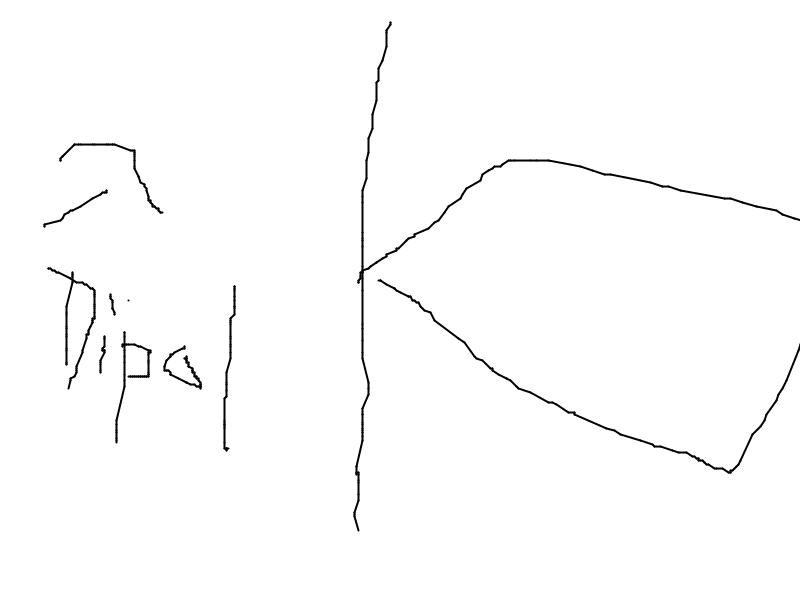
\includegraphics[width=\textwidth]{./example-image}
	\source{\cite{dipol_antenna}}
	\caption{Richtcharakteristik eine \(\lambda\)-Dipolantenne bei symmetrischer Einspeisung}
\end{figure}

\section{Zusammenfassung und Ausblicke}


%\bibliographystyle{plain}
\bibliography{cites}
\bibliographystyle{unsrtnat}
\end{document}
